\subsection{Exercício 1}
De forma a dar inicio ao estudo dos dados, é primeiramente nos pedido para que carreguemos o ficheiro \textbf{Clientes\_DataSet.csv} no ambiente R, verifiquemos a sua dimensão e obtenhamos um sumário dos dados. Recorrendo à função \textbf{csv} da biblioteca \textbf{read}, indicamos a localização do ficheiros e especificamos na variável opcional \textbf{head} que a primeira linha contém o nome das colunas. Por fim, armazenamos os dados na variável \textit{Clientes\_DataSet}, sobe a forma de um data frame. De seguida, obtemos a dimensão com a função \textbf{dim}, onde usamos \textit{Clientes\_DataSet} como parâmetro e obtemos os valores de \textit{7043} linhas e \textit{21} colunas. No contexto do sumário, recorrendo à função \textbf{summary} obtemos uma analise sobre cada coluna, sendo de destacar que as colunas em que os dados são números, é nos dado o detalhe sobre algumas medidas de localização, como podemos verificar para Fig. 2.

\begin{figure}[htbp]
\centerline{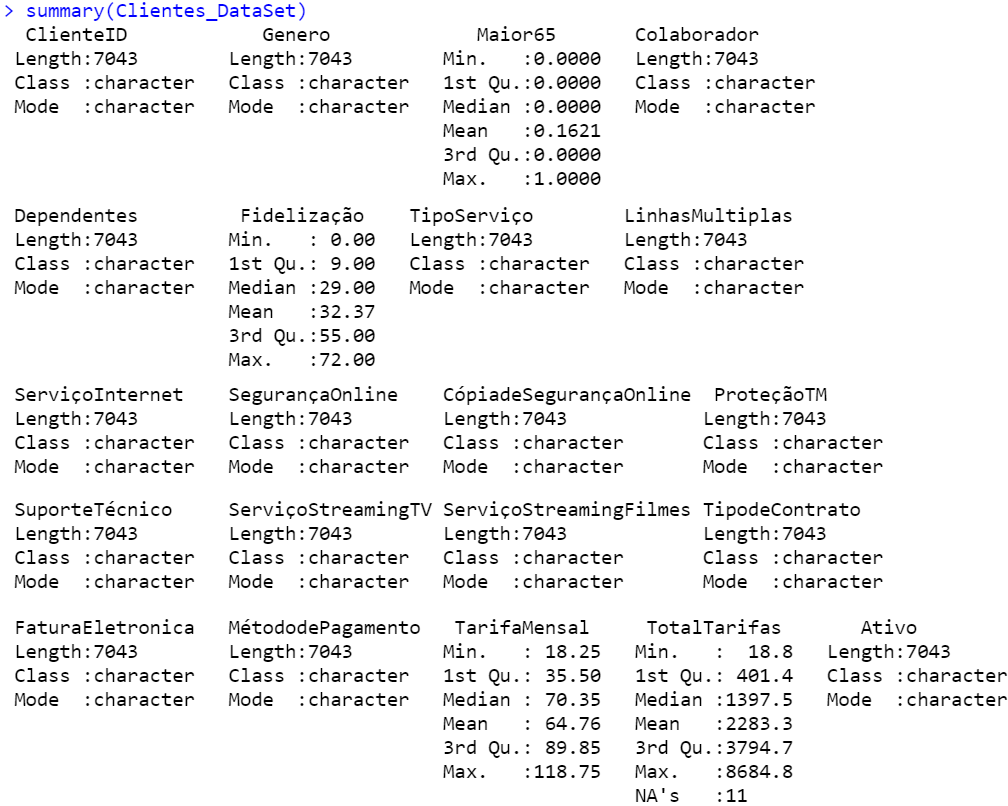
\includegraphics[width=9.5cm]{images/ex_1_summary2.png}}
\caption{Sumario do ficheiro Clientes\_DataSet.csv}
\label{ex_1_summary2}
\end{figure}

